\documentclass[numbering=fraction,10pt]{beamer}

\usepackage[utf8]{inputenc}
\usepackage[T1]{fontenc}
\usepackage[french]{babel}
\usepackage{blindtext}
\usepackage{tikzsymbols}
\usepackage{graphicx}
\usepackage{wrapfig}
\usepackage{bookman}
\usepackage{subcaption}
\usepackage[export]{adjustbox}



\usetheme[progressbar=frametitle]{metropolis}

%Define colors
\definecolor{wuppergreen}{RGB}{85, 171, 38}
\definecolor{background}{RGB}{255,255,255}

%Adding logo to title page
\titlegraphic{\raggedleft 
\includegraphics[width=3cm]{UNamur.png}}

%Adjust color theme
\setbeamercolor{frametitle}{bg=wuppergreen}
\setbeamercolor{title separator}{fg=wuppergreen}
\setbeamercolor{footline}{fg=gray}
\setbeamercolor{progress bar}{fg=black}

\setcounter{tocdepth}{1}

%Adding footer
\setbeamertemplate{frame footer}{\insertshortauthor~(\insertshortinstitute)}

\graphicspath{ {../Images/}}

%Set parameters for title page
\title{PIMS}
\author[PIMS]{Luis Dierick \and Gaillard Matthys \and Bouncer Yassine \and Fundu Oliver \and Anderson Rosny \and Tom Marchal }
\institute{Université de Namur}
\date{\today}

\begin{document}

\begin{frame}[plain]{}
    \maketitle
\end{frame}

\begin{frame}{Table des matières}
    \tableofcontents[]
\end{frame}
<<<<<<< HEAD
% Ne pas oublier d'expliquer rapidement comment on a procédé pour y arriver
% Expliquer les différentes étapes de la réalisation du projet
\section{Objectif de la mission}
\begin{frame}{Objectif de la mission}
    \begin{enumerate}
        \item Création d'une application web permettant la gestion de délivrables pour un cours donnés.
        \item Implémentation de la la gestion de la vie d'un délivrable (work)
        \item Implication de plusieurs acteurs : 
        \begin{itemize}
            \item Etudiant : Peut s'inscrire à un cours, voir les cours auxquels il est inscrit, voir les échéances pour un cours et déposer un délivrable.
            \item Professeur : Responsable d'un cours, ajouter des échéances, voir les délivrables déposés par les étudiants et les évaluer.
            \item Superviseur : Aide à la gestion d'un cours. Peut soumettre des sujets et procéde à des évluations
            \item Administrateur : Gère les utilisateurs au sens large, les cours et les ues.
        \end{itemize}
    \end{enumerate}
\end{frame}
=======

>>>>>>> 15a49e7e4c981d29ff3b5091e1706afe3d62e610
\section{Base de données}
\begin{frame}{Base de données}
    \begin{enumerate}
        \item Impléntée avec PostGreSQL
        \item Dispose de divers avantages
        \begin{itemize}
            \item Sécurité : Niveau de protection élevé (2 couches supplémentaires)
            \item Large choix de type de données diverses : texte, document, JSON, autre, \dots
            \item Rapidité : Permet de gérer de grandes quantités de données grâce à son architecture permettant des bases de données distribuées
        \end{itemize}
    \end{enumerate}
\end{frame}
\subsection{Schéma de la base de données}
\subsubsection{Schéma de la base de données - schéma relationnel}
\begin{frame}{Schéma de la base de données}
    \begin{figure}
        \centering
        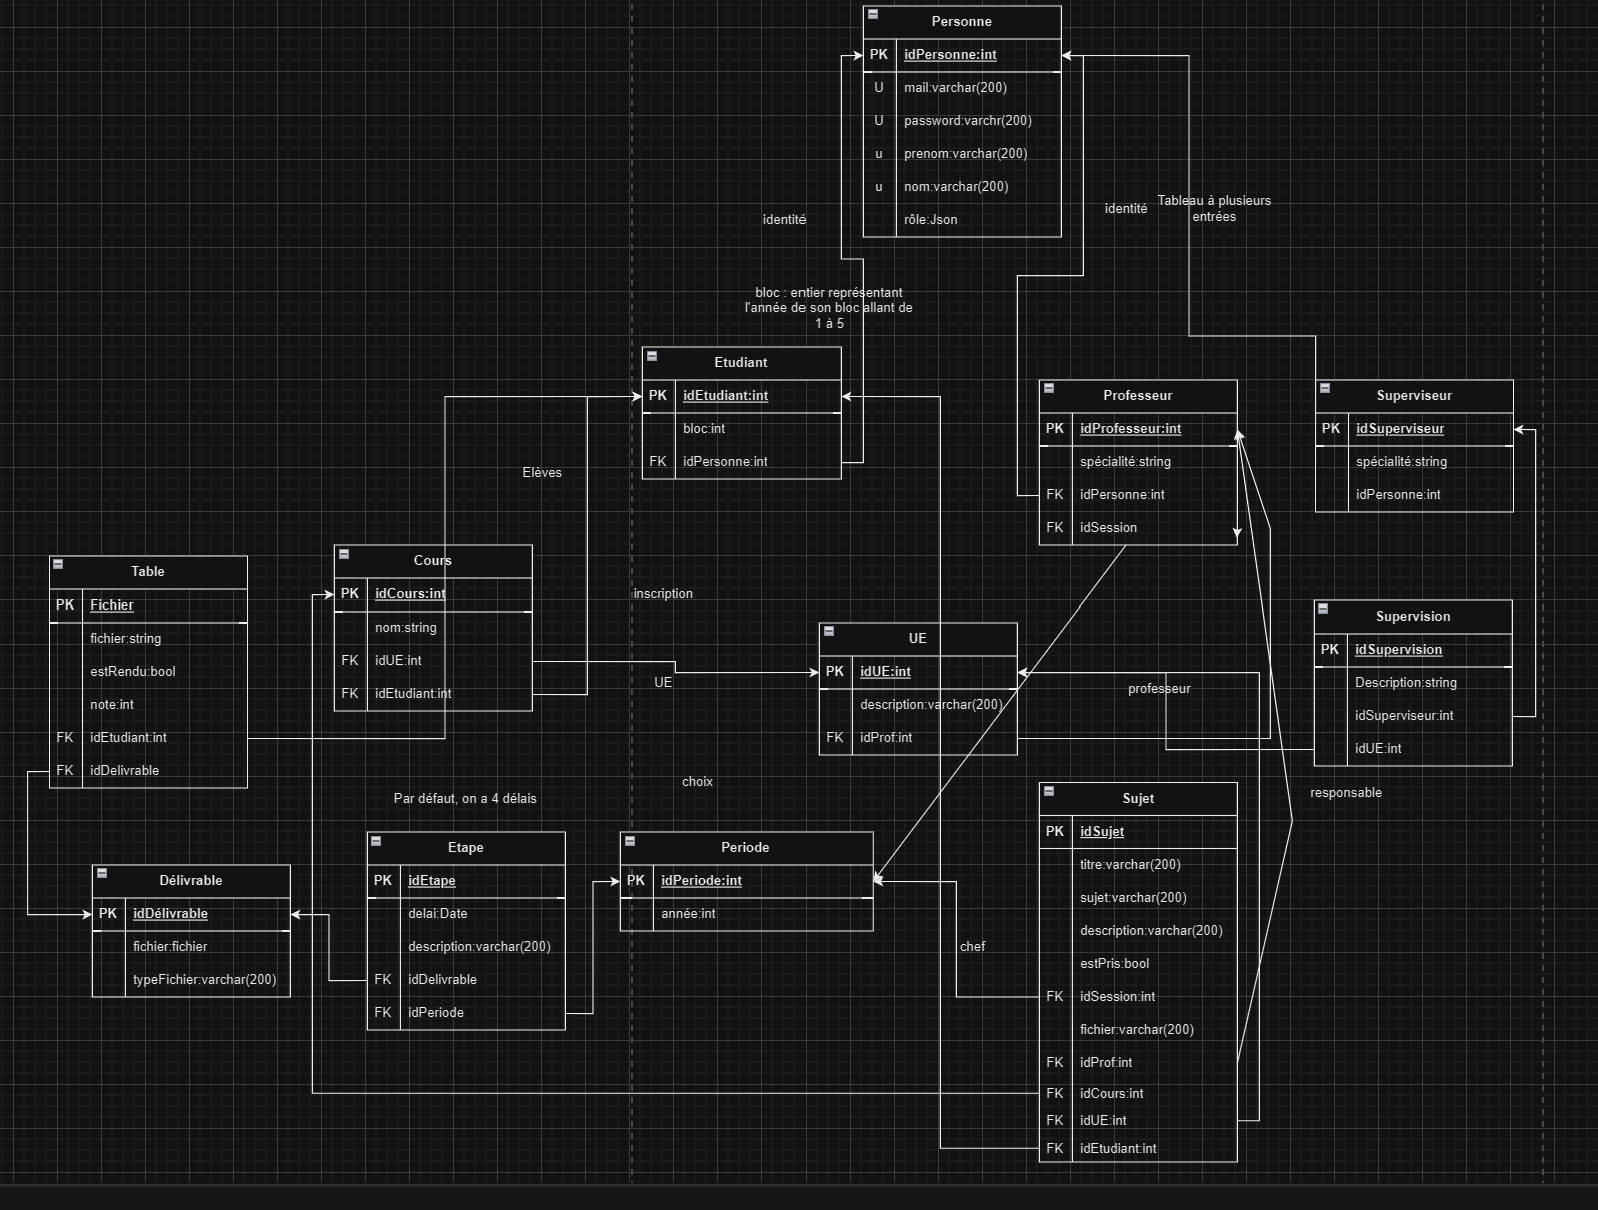
\includegraphics[width=0.8\textwidth]{dbrelation.png}
        \caption{Schéma de la base de données}
    \end{figure}
\end{frame}
\subsubsection{Schéma de la base de données - schéma entité-relation}
\begin{frame}{Schéma de la base de données- schéma entité-relation}
    \begin{figure}
        \centering
        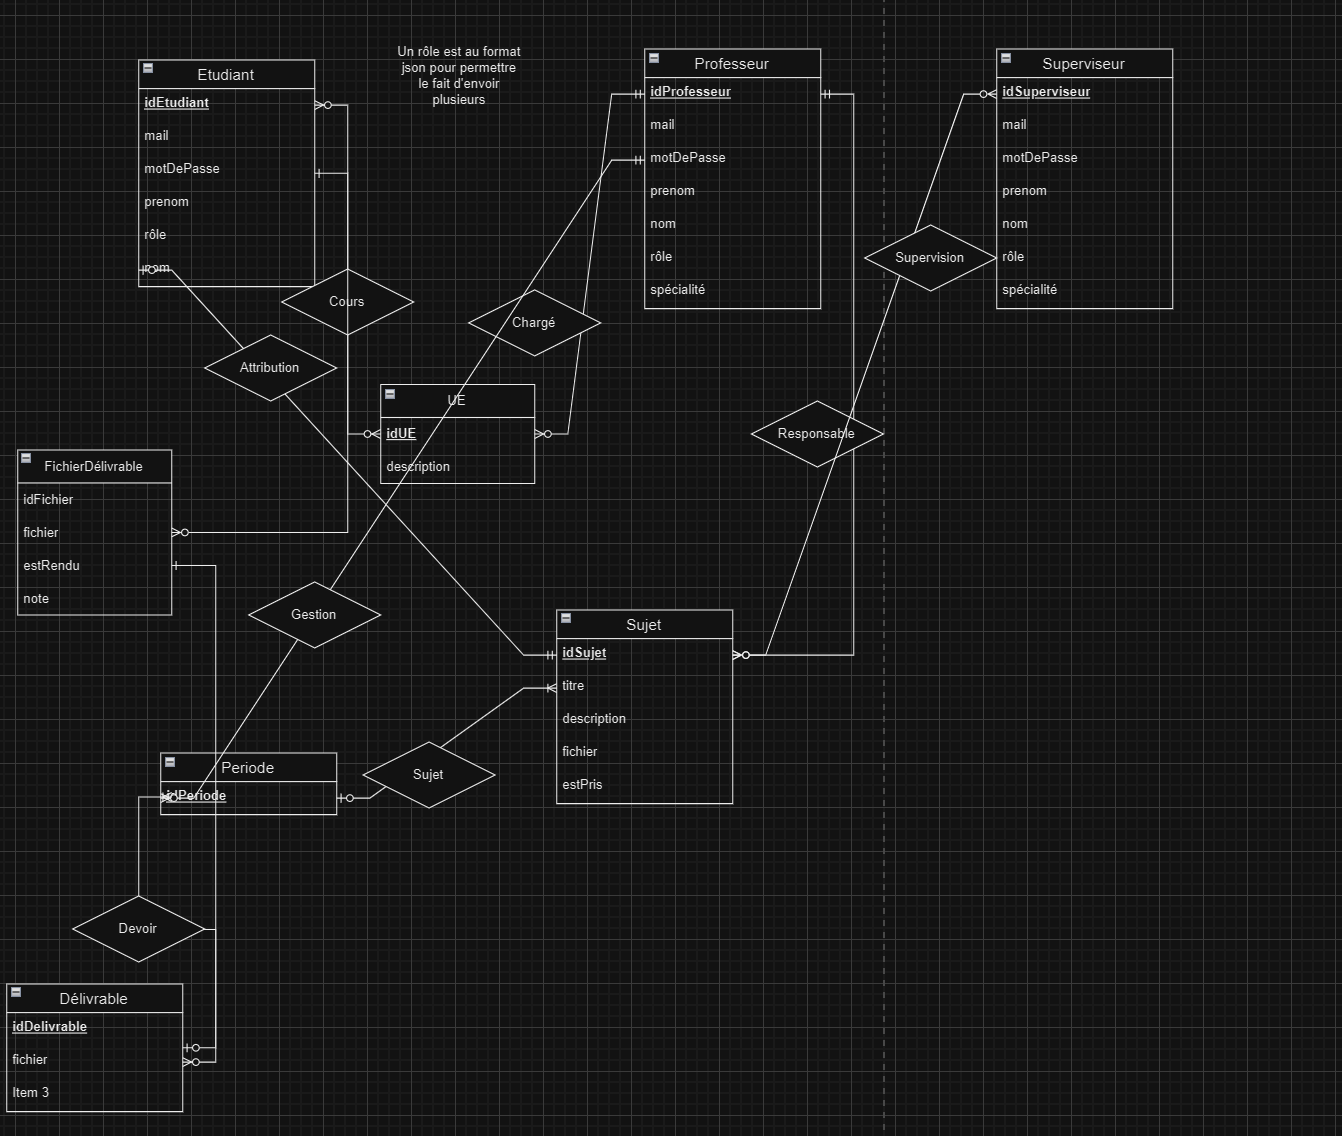
\includegraphics[width=0.8\textwidth]{dbER.png}
        \caption{Schéma de la base de données}
    \end{figure}
\end{frame}
\section{Méthode Agile}
\begin{frame}{Méthode Agile}
    \begin{figure}
        \centering
        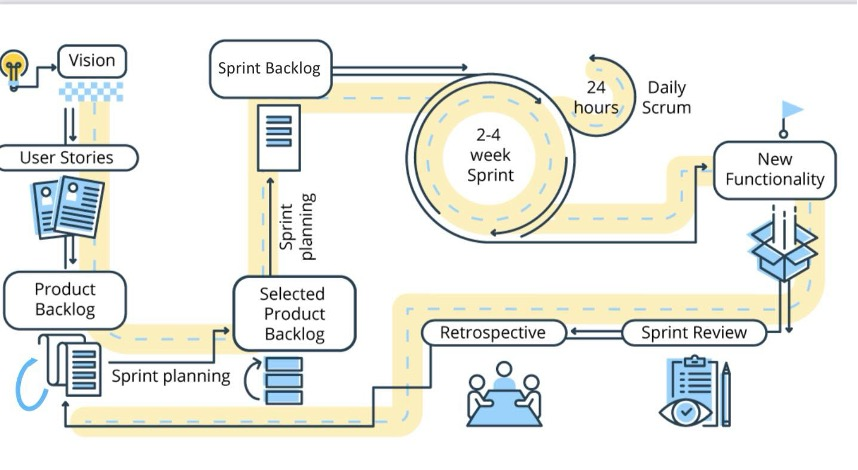
\includegraphics[width=0.8\textwidth]{agile.jpg}
        
    \end{figure}
\end{frame}
\section{Fonctionnalités}
\subsection{Fonctionnalités : Gestion des inscriptions à un cours}
\begin{frame}{Gestion des inscriptions à un cours}
    \begin{enumerate}
        \item Permet à un étudiant de s'inscrire à un cours
        \item Choix parmi toutes les ues disponibles
        \item Création d'une nouvelle occurrence de d'un cours
        \begin{itemize}
            \item Permet à un étudiant de s'inscrire à plusieurs cours
            \item Mécanisme permettant de gérer le fait qu'un étudiant ne peut pas s'inscrire à un cours déjà suivi
        \end{itemize}
        \item Choix via des cartes.
    \end{enumerate}
\end{frame}
\subsection{Fonctionnalités : Gestion des cours}
\begin{frame}{Gestion des cours}
    \begin{enumerate}
        \item Permets à un étudiant de voir les cours auquels il est inscrit.
        \item Visualisation grâce à des cartes.
        \item Clic permettant de voir les échéances pour un cours.
    \end{enumerate}
\end{frame}

\subsection{Vue d'ensemble}

\begin{frame}{Vue d'ensemble}
    \begin{itemize}
        \item Gestion des sujets
        \begin{itemize}
            \item CRUD
            \item Réservation
        \end{itemize} 
        \item Gestion des cours
        \begin{itemize}
            \item Modalités 
            \item Timeline + milestones
        \end{itemize}
        \item Interface dédiée aux administrateurs
        \begin{itemize}
            \item Gestion des rôles
            \item Archivage 
            \item Initialisation de la plateforme
        \end{itemize}
    \end{itemize}
\end{frame}


\begin{frame}{Pourquoi PIMS ?}
    \begin{itemize}
        \item Technologies modernes
        \item Plateforme synchronisée, automomatisée
        \item Vues adaptatives par rapport aux rôles
        \item[$\Longrightarrow$] \textbf{Facilité d'utilisation}
    \end{itemize}
\end{frame}


\end{document}  